\chapter{State of the art Survey}

\section{Introduction}
This chapter introduce all the different technologies currently available which deal with anonymity and privacy. Some of the technologies are already commercially available and being used in the industry, while some are still in research phase. We will give a brief introduction for all of them and brief idea how they can be used.


\section{Definitions and Common Terminology}
In this thesis, we have used some terminologies and definitions. Some of the important ones are given below:
\subsection{Privacy}
Privacy is the ability of an individual to control the distribution of information about himself. An individual should be able to choose which information about him should remain secret and which information can be revealed.
\subsection{Anonymity}
Anonymity refers to ability of a user to not give any information about him at all to the system. An anonymous system doesn't have any identity of the user.
\subsection{Pseudonym}
Pseudonym is a name given to the user in pseudonymous systems. This name is given to hide the real identity of the user from the system. The system only knows the user by his pseudonym.
\subsection{User}
User is the end user of the system. Its the person who will go online and get the services.
\subsection{Bank}
Bank is the financial institution which provides online financial services to the user. 
\subsection{Third party}
A third party or trusted third party is the entity which is neither bank or the user in the system. A third party provides different services to banks or users and hence reducing the burden on them to setup all the infrastructure by themselves.
\subsection{Service}
Service is something that is provided to the user online by a system. It may include ability to login, check his account balance, Upload pictures, share spreadhseets etc.
\subsection{Unlinkability}
Unlinkability is the privacy property where its not possible to link 2 different entities to each other even though they are the same. 
\\
\\e.g. not be able to link 2 different sessions by the same user in the system.
\subsection{Revocation}
Revocation is the property where a user credential is revoked by user or some other authority. After revocation, this credential cannot be used for anything.
\subsection{Partial Information Disclosure}
Its the ability of a user to only disclose some partial information about himself to the system. e.g. a user might just want to disclose his last name to the system but not his full name.
\subsection{Legal Requirement}
A legal requirement is something that is required by the law. e.g. it may be required by the law for the bank to log all the customer data. Also sometimes in case of suspicious transactions bank maybe required legally to give the user identity to the relevant authorities.
\subsection{Conditional Anonymity Removal}
Its the ability of the system to remove anonymity of the user if some conditions that were set before are met. This is mainly used for escrow purposes.

\begin{figure}[h]
	\centering
	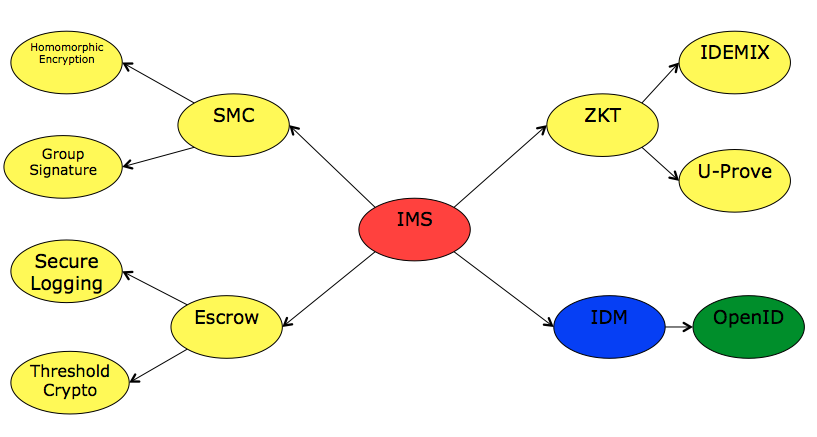
\includegraphics[width=\textwidth]{figures/Technologies}
	\caption{Technology Overview}
	\label{fig:Technologies}
\end{figure}
\section{Secure Multi-Party Computing}
These technologies are the ones which involve multiple parties to do computations. It is a subfield of cryptography which involves multiple parties getting an input and compute a joint function on them while keeping these inputs private. We basically looked at 2 technologies of interest here:
\subsection{Homomorphic Encryption}
Homomorphic encryption is a type of encryption where certain arithmetic operations can be performed on the ciphertext such that when the resultant ciphertext is decrypted, the decrypted text is same as the operations were performed on the plaintext. This is a new field of cryptography and is very useful where we need some parties to perform such operations without revealing the underlying data to those parties. Homomorphic encryption is also useful for chaining of different services without exposing data to any of those services.
\subsection{Group Signature}
A group signature is a scheme which allows a member of the group to sign the message on behalf of the group but anonymously. To outsiders the message has been signed by someone from the group but the exact identity of the person is now known. Also if the same member signs 2 different messages its not possible to know if the message is signed by the same member. There is a notion of group manager in these scheme. Group manager is someone who manages the membership to the group. He can add/remove members from the group, find out who actually signed the message from the group. This scheme is useful where only thing that needs to be validated is that a certain person is part of the group, but his real identity is not required.
\section{Escrow Technologies}
Escrow technologies are the ones which are helpful in escrow purposes i.e. getting real data/identity later on in time from encrypted data if needed. We look at following 2 technologies.
\subsection{Secure Logging}
Secure logging is the process of saving the data in a secure manner. As saved data is really crucial and vulnerable to the attacks. We need to make sure that data is saved securely and its integrity is protected. This can be done in several ways. One way is to encrypt all the logs while storing them so that even if someone get hold of the logs, they can't use them without having access to the decryption key. Other way is to store logs at a third party after encrypting them. For escrow purposes, these logs can be decrypted later on with the decryption key.
\subsection{Threshold Cryptography}
Threshold cryptography is a field of public key cryptography where in order to decrypt an encrypted message, several parties must cooperate in the decryption. This message is encrypted using a public key and the corresponding private key is shared among different parties who will participate in the decryption process i.e. multiple parties hold the private key for a single public key. There is a term called threshold, and if there are \textit{n} parties who share the private key and at least \textit{t} parties which are required to decrypt the message such system is called (t,n) threshold cryptosystem. Threshold cryptosystem is useful in escrow purposes where a minimum number of parties can be defined to decrypt the ciphertext in order to get the plaintext.

\section{Identity Management Systems}
These are traditional identity management systems. For our purposes we look at OpenID system.
\subsection{OpenID}
OpenID is an open and decentralized protocol, which can be used to authenticate to different co-operating sites with the use of a third party service. It has notion of a \textit{relying party} and \textit{OpenID identity provider}.
\begin{itemize}
\item \textbf{OpenID Identity Provider} OpenID identity provider is the service, which actually provides authentication services. End user registers at OpenID identity provider to get his OpenID identity.
\item \textbf{Relying Party} Relying party is the website which user wants to authenticate to and which rely on the OpenID identity provider to provide authentication.
\end{itemize}
In addition to this an extension called \textit{OpenID attribute exchange} helps facilitate the transfer of user attributes from identity provider to the relying party
\begin{itemize}
\item User goes to the relying party service page
\item Service page presents different OpenID providers to login to the service
\item User chose the provider he has registered his openID with
\item Relying party redirects the user to the OpenID provider url so that user can authenticate
\item User can be authenticated by the method provided by OpenID provider
\item OpenID provider asks user the permission to share the attributes with the relying party
\item After user consent, user is redirected to the relying party website with user credentials
\item Relying party can verify the credentials and then login the user to the service
\end{itemize}
\section{Zero Knowledge Technologies}
These are the technologies which use the concept of zero knowledge i.e. proving knowledge about something without divulging the information. For our purpose we focus on mainly 2 technologies – IDEMIX and U-Prove, which are based on the concept of zero knowledge and verifiable encryption.. They both have a lot in common and have been studied a lot in industry. 
\subsection{IDEMIX}
U-Prove is a digital credential technology by IBM. it relies on anonymous credentials known as IDEMIX tokens. It is based on Camenisch-Lysyanskaya (CL) signature scheme which provides efficient zero-knowledge proofs. IDEMIX  have different entities in the system
\begin{itemize}
	\item \textbf{User} User is basically the entity, which is proving his identity in the system.
	\item \textbf{Verifier} Verifier is the entity, which verifies the identity of the prover.
	\item \textbf{Issuer} Issuer is the entity, which issues the credentials to the prover to prove his identity
	\item \textbf{Inspector} Inspector is the entity, which in case of discrepancy or legal requirement , can actually come and get the real identity of the prover.
\end{itemize}
\begin{figure}[h]
	\centering
	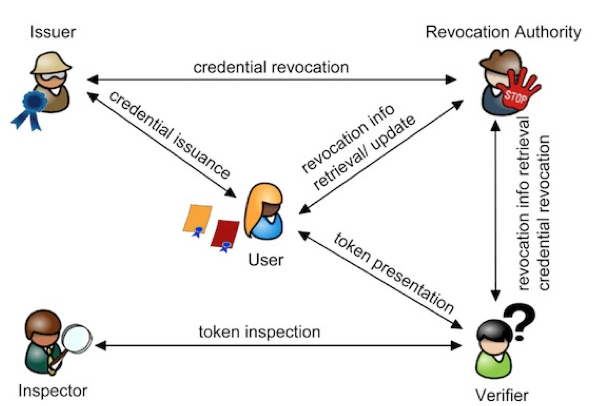
\includegraphics[width=\textwidth]{figures/Roles}
	\begin{minipage}{\textwidth}
		\footnotesize
		\emph{Source: https://github.com/p2abcengine/p2abcengine/wiki/Concepts-and-features}
	\end{minipage}
	\caption{IDEMIX Roles}
	\label{fig:Roles}
\end{figure}

For IDEMIX we need computing devices which work on behalf of each entity in the system.
\subsubsection{IDEMIX Credential}
An Idemix credential is CL Signature by issuer on user's private key and on attribute values. A user have independent public keys or pseudonyms for the same private key. These pseudonyms are IDEMIX tokens which are then used by the user to prove his identity to the different verifiers. IDEMIX has been studied a lot and many EU projects on anonymous credentials are based on it e.g. FutureID, ABC4Trust etc.
\begin{figure}[h]
	\centering
	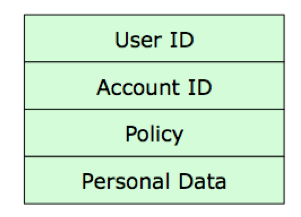
\includegraphics[width=170pt]{figures/Credential}
	\caption{IDEMIX Credential}
	\label{fig:Credential}
\end{figure}
\subsubsection{Issuance}
The first step is the credential issuance. It involves following steps:
\begin{itemize}
	\item User sends credential request to the issuer
	\item Issuer presents the issuance policy specifying
		\subitem Which attributes to present
		\subitem Which pseudonym/existing credentials to present
	\item Issuer also present a credential template specifying
		\subitem Which attributes of the new credentials will be generated at random
		\subitem Or carried over from existing credential or pseudonym
	\item User then present the issuance token satisfying the issuance policy
	\item Then multi-round cryptographic protocol ensues at end of which user get the IDEMIX credential
\end{itemize}
\subsubsection{Presentation}
Next step is to present the IDEMIX token for authentication to the verifier. It consists of following steps:
\begin{figure}[h]
	\centering
	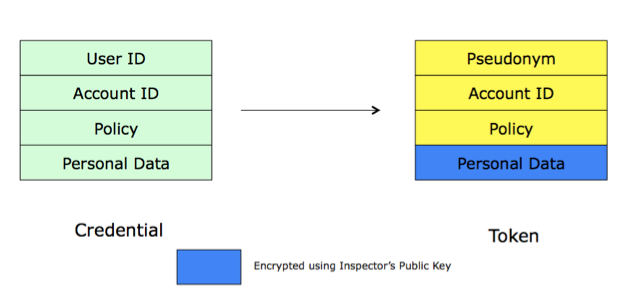
\includegraphics[width=\textwidth]{figures/Token}
	\caption{IDEMIX Presentation Token}
	\label{fig:Token}
\end{figure}
\begin{itemize}
	\item User get the presentation policy from the verifier which specifies
		\subitem Which credentials user must present
		\subitem What information user should reveal from these credential
	\item User generate a presentation token in accordance with the presentation policy revealing only the attributes necessary
	\item User present this presentation token to the verifier
	\item Verifier can then verify the attributes
\end{itemize}
\subsubsection{ID Escrow}
IDEMIX provides the ID escrow ability in case it is required. Following steps need to be followed for ID escrow purposes in IDEMIX:
\begin{itemize}
	\item The presentation policy can have following optional specifications for the purpose of ID Escrow
	\begin{itemize}
		\item Public keys of inspectors
		\item Attributes values to be encrypted using the keys	
		\item Inspection conditions under which these attributes can be revealed
	\end{itemize}
	\item User can prove that he has put these values in the presentation token with verifiable encryption to the verifier
	\item Once the token in presented, the inspection conditions are fixed and cannot be changed 
	\item In case of some discrepancy or legal requirement, an inspector can come and get the identity of the user from the token
\end{itemize}


\subsection{U-Prove}
U-Prove is a digital credential technology by Microsoft. It relies on anonymous credentials known as U-Prove tokens. It provides users a way to minimaly disclose their personal information while interacting with different online services. U-prove have different entities in the system
\begin{itemize}
	\item \textbf{Prover} Prover is basically the entity, which is proving his identity in the system.
	\item \textbf{Verifier} Verifier is the entity, which verifies the identity of the prover.
	\item \textbf{Issuer} Issuer is the entity, which issues the credentials to the prover to prove his identity
	\item \textbf{Auditor} Auditor is the entity, which in case of discrepancy or legal requirement , can actually come and get the real identity of the prover.
\end{itemize}
For U-Prove we need computing devices which work on behalf of each entity in the system.
\subsubsection{U-Prove Token}
U-Prove token is basically cryptographically protected information of any kind e.g. attributes. These are issued by issuer to the prover by issuance protocol. These tokens are then presented by prover to the verifier. Issuance and presentation of U-Prove tokens is unlinkable.
\subsubsection{Issuance}
The first step is the credential issuance. It involves following steps:
\begin{itemize}
	\item Prover invoke U-Prove issuance protocol
	\item Prover provides the attributes to be encoded
	\subitem Using \textit{Collaborative Issuance} property user can make sure that issuer doesn’t actually knows the attributes
	\item Then multi-round cryptographic protocol ensues at end of which user get the U-Prove token from the issuer
\end{itemize}
\subsubsection{Presentation}
Next step is to present the U-Prove token for authentication to the verifier. It consists of following steps:
\begin{itemize}
	\item Prover invoke the U-Prove presentation protocol
	\item User generate a presentation token in accordance with the presentation policy revealing only the attributes necessary
	\item User present this presentation token to the verifier
	\item Verifier can then verify the attributes
\end{itemize}
It must be noted that a revocation check can be added if needed before verifying the token.
\subsubsection{ID Escrow}
ID Escrow in U-Prove is actually an extension to existing U-Prove technology. It uses a type of ElGamal encryption which is verifiable.
\begin{itemize}
	\item  During the presentation protocol, prover proves that his ID is encrypted in the token by the use of verifiable encryption technology
	\item De-anonymization cannot be done by verifier or issuer
	\item A special entity called Auditor is responsible for de-anonymization in case of some discrepancy or legal requirement
	\item Threshold cryptography can be used in case of auditors and key can be split among multiple auditors.
\end{itemize}
\section{Summary}
All these different technologies provide different level of anonymization in the system. Some of them are easy to integrate in existing technology, while some are still not mature enough. For our purposes from now on we focus on mainly 2 technologies:
\begin{itemize}
	\item OpenID
	\item IDEMIX
\end{itemize}